\chapter{Page Replacement Algorithms}

\section{Introduction}

Virtual memory allows processes to execute even when their entire address space is not loaded into physical memory. Since physical memory is limited, the operating system must decide which page should be removed when a new page needs to be loaded.

This decision is made by a \textbf{Page Replacement Algorithm}.

Page replacement is one of the most important interview topics in Operating Systems because it combines theory, numerical problem solving, performance analysis, and system design considerations.

\section{Learning Objectives}

After studying this chapter, you should be able to:

\begin{itemize}
\item Explain why page replacement is necessary.
\item Calculate page faults for common algorithms.
\item Analyze reference strings.
\item Compare replacement algorithms.
\item Understand Belady's Anomaly.
\item Solve page replacement numericals quickly.
\item Discuss practical implementations in modern operating systems.
\end{itemize}

%====================================================
\section{Why Page Replacement is Needed}
%====================================================

When a process accesses a page that is not currently in memory:

\begin{enumerate}
\item A page fault occurs.
\item OS loads the required page.
\item If all frames are occupied, a page must be removed.
\end{enumerate}

The choice of which page to remove directly affects performance.

\subsection{Example}

Available Frames:

[
3
]

Current Pages:

[
[1,2,3]
]

Incoming Page:

[
4
]

One page must be evicted.

\section{Frame Allocation Basics}

\subsection{Frame}

A frame is a fixed-size block in physical memory.

\subsection{Page}

A page is a fixed-size block in virtual memory.

\subsection{Relationship}

[
Page \rightarrow Frame
]

Each loaded page occupies exactly one frame.

\subsection{Allocation Strategies}

\begin{itemize}
\item Equal Allocation
\item Proportional Allocation
\item Priority-Based Allocation
\end{itemize}

\section{Page Faults}

\subsection{Definition}

A page fault occurs when a referenced page is not present in memory.

\subsection{Steps}

\begin{enumerate}
\item Trap to OS.
\item Locate page on disk.
\item Select victim page.
\item Load required page.
\item Resume execution.
\end{enumerate}

\subsection{Impact}

Page faults are expensive because disk access is much slower than RAM access.

\section{Reference Strings}

\subsection{Definition}

A reference string is a sequence of page references generated by a process.

\subsection{Example}

[
7,0,1,2,0,3,0,4,2,3,0,3,2
]

This sequence is used to analyze replacement algorithms.

\section{Performance Considerations}

Important metrics include:

\begin{itemize}
\item Number of page faults
\item Hit ratio
\item Miss ratio
\item CPU utilization
\item Disk I/O overhead
\end{itemize}

\subsection{Goal}

Minimize page faults.

%====================================================
\section{FIFO (First-In First-Out)}
%====================================================

\subsection{Theory}

The oldest loaded page is replaced first.

\subsection{Working Principle}

Pages are maintained in queue order.

\subsection{Example}

Frames = 3

Reference String:

[
1,2,3,4
]

Memory Evolution:

[
[1]
]

[
[1,2]
]

[
[1,2,3]
]

[
[4,2,3]
]

Page 1 is removed first.

\subsection{Advantages}

\begin{itemize}
\item Very simple
\item Easy implementation
\end{itemize}

\subsection{Disadvantages}

\begin{itemize}
\item Ignores usage history
\item Suffers from Belady's Anomaly
\end{itemize}

\subsection{Complexity}

[
O(1)
]

with queue implementation.

%====================================================
\section{Optimal Page Replacement}
%====================================================

\subsection{Theory}

Replace the page that will not be used for the longest future duration.

\subsection{Example}

Frames = 3

Reference String:

[
7,0,1,2
]

Current Memory:

[
7,0,1
]

Incoming Page:

[
2
]

Future references indicate page 7 is never used again.

Replace page 7.

\subsection{Advantages}

\begin{itemize}
\item Minimum possible page faults
\item Benchmark algorithm
\end{itemize}

\subsection{Disadvantages}

\begin{itemize}
\item Requires future knowledge
\item Not implementable in practice
\end{itemize}

\subsection{Complexity}

[
O(n)
]

future scan per replacement.

%====================================================
\section{LRU (Least Recently Used)}
%====================================================

\subsection{Theory}

Replace the page that has not been used for the longest time in the past.

\subsection{Example}

Frames:

[
[2,3,4]
]

Recent Usage:

[
4,3,2
]

Page 2 is least recently used.

Replace page 2.

\subsection{Advantages}

\begin{itemize}
\item Good practical approximation
\item Stack algorithm
\end{itemize}

\subsection{Disadvantages}

\begin{itemize}
\item Tracking history is expensive
\end{itemize}

\subsection{Complexity}

[
O(1)
]

with specialized hardware support.

%====================================================
\section{Second Chance Algorithm}
%====================================================

\subsection{Theory}

FIFO enhanced with reference bits.

\subsection{Working}

If Reference Bit = 1:

\begin{itemize}
\item Clear bit
\item Give page another chance
\end{itemize}

If Reference Bit = 0:

Replace page.

\subsection{Advantages}

\begin{itemize}
\item Better than FIFO
\item Simple implementation
\end{itemize}

\subsection{Disadvantages}

\begin{itemize}
\item Approximation only
\end{itemize}

\subsection{Complexity}

Approximately:

[
O(1)
]

Average case.

%====================================================
\section{Clock Algorithm}
%====================================================

\subsection{Theory}

Efficient implementation of Second Chance.

\subsection{Structure}

Pages arranged in circular form.

\begin{figure}[h]
\centering
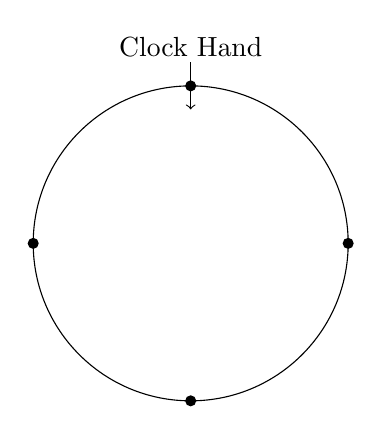
\begin{tikzpicture}
\draw (0,0) circle (2cm);

\node at (0,2.5) {Clock Hand};

\fill (2,0) circle (2pt);
\fill (-2,0) circle (2pt);
\fill (0,2) circle (2pt);
\fill (0,-2) circle (2pt);

\draw[->] (0,2.3)--(0,1.7);
\end{tikzpicture}
\caption{Clock Page Replacement}
\end{figure}

\subsection{Advantages}

\begin{itemize}
\item Efficient
\item Widely used
\end{itemize}

\subsection{Disadvantages}

\begin{itemize}
\item Approximate LRU
\end{itemize}

\section{Enhanced Clock Algorithm}

\subsection{Theory}

Uses:

\begin{itemize}
\item Reference Bit (R)
\item Modified Bit (M)
\end{itemize}

\subsection{Priority Order}

[
(0,0)
]

[
(0,1)
]

[
(1,0)
]

[
(1,1)
]

Pages with lowest priority are replaced first.

\subsection{Advantages}

\begin{itemize}
\item Considers dirty pages
\item Better decisions
\end{itemize}

\subsection{Disadvantages}

\begin{itemize}
\item More complexity
\end{itemize}

%====================================================
\section{LFU (Least Frequently Used)}
%====================================================

\subsection{Theory}

Replace page with lowest access frequency.

\subsection{Example}

Frequency Counts:

[
P1=10
]

[
P2=3
]

[
P3=7
]

Replace:

[
P2
]

\subsection{Advantages}

\begin{itemize}
\item Uses long-term history
\end{itemize}

\subsection{Disadvantages}

\begin{itemize}
\item Old references dominate
\end{itemize}

\subsection{Complexity}

[
O(\log n)
]

using priority queues.

%====================================================
\section{MFU (Most Frequently Used)}
%====================================================

\subsection{Theory}

Replace the page with highest access count.

\subsection{Idea}

Frequently used pages may have completed their purpose.

\subsection{Advantages}

Useful in specialized workloads.

\subsection{Disadvantages}

Generally performs worse than LRU.

\subsection{Complexity}

[
O(\log n)
]

%====================================================
\section{NRU (Not Recently Used)}
%====================================================

\subsection{Theory}

Uses:

\begin{itemize}
\item Reference Bit
\item Modified Bit
\end{itemize}

Pages classified into four classes.

\subsection{Classes}

[
(0,0)
]

[
(0,1)
]

[
(1,0)
]

[
(1,1)
]

Replace lowest class page.

\subsection{Advantages}

\begin{itemize}
\item Simple approximation
\end{itemize}

\subsection{Disadvantages}

\begin{itemize}
\item Coarse-grained decisions
\end{itemize}

%====================================================
\section{Random Replacement}
%====================================================

\subsection{Theory}

Select victim page randomly.

\subsection{Advantages}

\begin{itemize}
\item Extremely simple
\item No bookkeeping
\end{itemize}

\subsection{Disadvantages}

\begin{itemize}
\item Unpredictable performance
\end{itemize}

\subsection{Complexity}

[
O(1)
]

%====================================================
\section{Solved Numerical Example 1}
%====================================================

Frames = 3

Reference String:

[
1,2,3,4,1,2,5
]

FIFO Simulation:

\begin{center}
1 F

2 F

3 F

4 F

1 F

2 F

5 F
\end{center}

Total Page Faults:

[
7
]

%====================================================
\section{Solved Numerical Example 2}
%====================================================

Frames = 3

Reference String:

[
1,2,3,1,4,5
]

LRU Simulation:

Faults:

[
1,2,3,4,5
]

Total:

[
5
]

%====================================================
\section{Solved Numerical Example 3}
%====================================================

Frames = 4

Reference String:

[
7,0,1,2,0,3,0,4
]

Optimal replacement yields minimum page faults.

Result:

[
6
]

page faults.

%====================================================
\section{Belady's Anomaly}
%====================================================

\subsection{Definition}

Increasing the number of frames causes more page faults.

\subsection{Example}

FIFO:

Frames = 3

Page Faults = 9

Frames = 4

Page Faults = 10

More memory produced worse performance.

\subsection{Observation}

Occurs in:

\begin{itemize}
\item FIFO
\end{itemize}

Does not occur in:

\begin{itemize}
\item LRU
\item Optimal
\end{itemize}

%====================================================
\section{Stack Algorithms}
%====================================================

\subsection{Definition}

Algorithms where pages in (n) frames are always a subset of pages in (n+1) frames.

\subsection{Examples}

\begin{itemize}
\item LRU
\item Optimal
\end{itemize}

\subsection{Property}

Never exhibit Belady's Anomaly.

%====================================================
\section{Working Set Based Replacement}
%====================================================

\subsection{Theory}

Maintain set of pages actively used by a process.

\subsection{Working Set}

Pages referenced during recent interval.

[
W(t,\Delta)
]

\subsection{Advantages}

\begin{itemize}
\item Prevents thrashing
\item Good locality support
\end{itemize}

\subsection{Disadvantages}

\begin{itemize}
\item Tracking overhead
\end{itemize}

%====================================================
\section{Page Buffering}
%====================================================

\subsection{Definition}

Maintain pool of free frames for quick allocation.

\subsection{Benefits}

\begin{itemize}
\item Faster page fault handling
\item Reduced latency
\end{itemize}

\subsection{Working}

Victim pages moved to buffer before permanent removal.

%====================================================
\section{Algorithm Comparison}
%====================================================

\begin{table}[h]
\centering
\small
\begin{tabular}{|p{3cm}|p{2cm}|p{2cm}|p{4cm}|}
\hline
Algorithm & Optimality & Practical & Belady \
\hline
FIFO & Poor & Yes & Yes \
\hline
Optimal & Best & No & No \
\hline
LRU & Excellent & Yes & No \
\hline
Second Chance & Good & Yes & Rare \
\hline
Clock & Good & Yes & Rare \
\hline
Enhanced Clock & Better & Yes & Rare \
\hline
LFU & Moderate & Limited & No \
\hline
MFU & Moderate & Limited & No \
\hline
NRU & Moderate & Yes & No \
\hline
Random & Weak & Yes & No \
\hline
\end{tabular}
\caption{Page Replacement Comparison}
\end{table}

%====================================================
\section{Interview Shortcuts}
%====================================================

\subsection{Shortcut 1}

Optimal always gives minimum page faults.

\subsection{Shortcut 2}

LRU is a stack algorithm.

\subsection{Shortcut 3}

FIFO may exhibit Belady's Anomaly.

\subsection{Shortcut 4}

Clock = Efficient Second Chance.

\subsection{Shortcut 5}

Working Set helps prevent thrashing.

%====================================================
\section{Key Takeaways}
%====================================================

\begin{itemize}
\item Page replacement handles full memory situations.
\item FIFO is simple but imperfect.
\item Optimal provides theoretical lower bound.
\item LRU is widely used.
\item Clock approximates LRU efficiently.
\item LFU uses frequency information.
\item NRU uses reference and modify bits.
\item Belady's Anomaly affects FIFO.
\item Stack algorithms avoid Belady's Anomaly.
\item Working Set reduces thrashing.
\end{itemize}

%====================================================
\section{25 Interview Questions with Answers}
%====================================================

\begin{enumerate}
\item What is page replacement?\
Answer: Selecting a victim page during page faults.

\item Why is page replacement needed?\
Answer: Physical memory is limited.

\item What is a page fault?\
Answer: Referenced page not present in memory.

\item What is a frame?\
Answer: Physical memory block.

\item What is FIFO?\
Answer: First-In First-Out replacement.

\item FIFO disadvantage?\
Answer: Belady's Anomaly.

\item What is Optimal replacement?\
Answer: Replace farthest future page.

\item Why is Optimal impractical?\
Answer: Future knowledge unavailable.

\item What is LRU?\
Answer: Least Recently Used.

\item LRU approximates what principle?\
Answer: Temporal locality.

\item What is Second Chance?\
Answer: FIFO with reference bits.

\item What is Clock algorithm?\
Answer: Circular Second Chance.

\item Enhanced Clock uses which bits?\
Answer: Reference and Modified.

\item LFU means?\
Answer: Least Frequently Used.

\item MFU means?\
Answer: Most Frequently Used.

\item NRU means?\
Answer: Not Recently Used.

\item What is Random replacement?\
Answer: Random victim selection.

\item What is Belady's Anomaly?\
Answer: More frames causing more faults.

\item Which algorithm suffers from Belady?\
Answer: FIFO.

\item What is a stack algorithm?\
Answer: Subset property algorithm.

\item Give stack algorithm examples.\
Answer: LRU, Optimal.

\item Working Set purpose?\
Answer: Prevent thrashing.

\item What is page buffering?\
Answer: Maintain free-frame pool.

\item Best theoretical algorithm?\
Answer: Optimal.

\item Most commonly discussed practical algorithm?\
Answer: LRU.
\end{enumerate}

%====================================================
\section{25 MCQs with Answers}
%====================================================

\begin{enumerate}
\item FIFO stands for:
Answer: First In First Out

\item LRU stands for:
Answer: Least Recently Used

\item LFU stands for:
Answer: Least Frequently Used

\item MFU stands for:
Answer: Most Frequently Used

\item NRU stands for:
Answer: Not Recently Used

\item Optimal replacement requires:
Answer: Future knowledge

\item Page fault occurs when:
Answer: Page absent from memory

\item Frame belongs to:
Answer: Physical Memory

\item Page belongs to:
Answer: Virtual Memory

\item FIFO suffers from:
Answer: Belady's Anomaly

\item LRU is:
Answer: Stack Algorithm

\item Optimal is:
Answer: Stack Algorithm

\item Clock is based on:
Answer: Second Chance

\item Enhanced Clock uses:
Answer: R and M bits

\item Working Set helps prevent:
Answer: Thrashing

\item Random replacement complexity:
Answer: O(1)

\item LRU exploits:
Answer: Temporal Locality

\item FIFO uses:
Answer: Queue

\item LFU uses:
Answer: Frequency Count

\item Optimal gives:
Answer: Minimum Faults

\item Belady's anomaly affects:
Answer: FIFO

\item Page buffering improves:
Answer: Fault Handling

\item NRU classification uses:
Answer: Two Bits

\item Clock structure is:
Answer: Circular

\item Best benchmark algorithm:
Answer: Optimal
\end{enumerate}

%====================================================
\section{Revision Notes}
%====================================================

\begin{itemize}
\item Page replacement occurs after page faults.
\item FIFO removes oldest page.
\item Optimal removes farthest future page.
\item LRU removes least recently used page.
\item Clock approximates LRU.
\item LFU uses access frequency.
\item NRU uses reference and modified bits.
\item FIFO may show Belady's Anomaly.
\item LRU and Optimal are stack algorithms.
\item Working Set helps prevent thrashing.
\end{itemize}

%====================================================
\section{Cheat Sheet}
%====================================================

\begin{center}
\begin{tabular}{|p{5cm}|p{8cm}|}
\hline
FIFO & Oldest Page First \
\hline
Optimal & Farthest Future Use \
\hline
LRU & Least Recent Use \
\hline
Second Chance & FIFO + Reference Bit \
\hline
Clock & Circular Second Chance \
\hline
Enhanced Clock & R Bit + M Bit \
\hline
LFU & Lowest Frequency \
\hline
MFU & Highest Frequency \
\hline
NRU & Not Recently Used \
\hline
Random & Random Victim \
\hline
Belady's Anomaly & More Frames, More Faults \
\hline
Stack Algorithms & LRU, Optimal \
\hline
Working Set & Active Pages \
\hline
Page Buffering & Free Frame Pool \
\hline
Goal & Minimize Page Faults \
\hline
\end{tabular}
\end{center}
